%%%%%%%%%%%%%%%%%%%%%%%%%%%%%%%%%%%%%%%%%%%%%%%%%%%%%%%%%%%%%%%%%%%%%%%%%%%%%%%
\chapter{Pesquisa em memória primária}
%%%%%%%%%%%%%%%%%%%%%%%%%%%%%%%%%%%%%%%%%%%%%%%%%%%%%%%%%%%%%%%%%%%%%%%%%%%%%%%

A pesquisa ocorre em uma estrutura de dados armazenada em memória principal e
a informação é dividida em registros com {\bf chaves de busca}.
O objetivo da pesquisa é encontrar uma ou mais ocorrências de registros com
chave de busca igual a chave usada na pesquisa.

O armazenamento dos dados é em geral feita por {\bf vetores} e/ou {\bf listas
encadeadas} (pesquisa sequencial e pesquisa binária), ou {\bf árvores de
pesquisa binária} (árvores com ou sem balanceamento).

%%%%%%%%%%%%%%%%%%%%%%%%%%%%%%%%%%%%%%%%%%%%%%%%%%%%%%%%%%%%%%%%%%%%%%%%%%%%%%%
\section{Pesquisa sequencial}
%%%%%%%%%%%%%%%%%%%%%%%%%%%%%%%%%%%%%%%%%%%%%%%%%%%%%%%%%%%%%%%%%%%%%%%%%%%%%%%

A {\bf pesquisa sequencial} (ou força-bruta) é o método de pesquisa mais
simples e lê todos os dados a partir do início do vetor e compara com a chave
de busca até encontrar um registro ou até o final do vetor.
A lógica de busca depende da ordenação dos dados e da possibilidade de existirem
chaves repetidas.

Alguns exemplos de busca são:
\begin{itemize}
\item dados {\bf não ordenados} e chaves {\bf repetidas} - deve-ser
varrer todos os registros.

\item dados {\bf não ordenados} e chaves {\bf não repetidas} - 
deve-se varrer todos os registros até encontrar a chaves buscada.

\item dados {\bf ordenados} e chaves {\bf repetidas} -
deve-se varrer todos os registros até encontrar alguma chave maior 
do que a buscada.
No caminho, vários registros podem ser encontrados.

\item dados {\bf ordenados} e chaves {\bf não repetidas} -
deve-se varrer todos os registros até encontrar alguma chave maior 
do que a buscada.
No caminho, um registro pode ser encontrado.

\end{itemize}

O custo médio da pesquisa sequencial é medido em função do número de acessos
feitos em cada busca.
No caso da busca sem sucesso (não ordenado e não repetido) o custo é $C(n) =
n+1$.
Quando tiver sucesso (não ordenado e não repetido)  o melhor caso é $C(n) = 1$,
pior caso $C(n)=n$ e caso médio $C(n) = (n+1)/2$.

%%%%%%%%%%%%%%%%%%%%%%%%%%%%%%%%%%%%%%%%%%%%%%%%%%%%%%%%%%%%%%%%%%%%%%%%%%%%%%%
\section{Pesquisa binária}
%%%%%%%%%%%%%%%%%%%%%%%%%%%%%%%%%%%%%%%%%%%%%%%%%%%%%%%%%%%%%%%%%%%%%%%%%%%%%%%

A {\bf busca binária} pode ser feito em vetores ou listas em que os elementos
devem estar {\bf em ordem}.

Os passos envolvidos na buca binária são:
\begin{enumerate}
\item Compare a chave com o registro que está na posição do meio do vetor.

\item Se a chave é menor, o registro procurado está na primeira metade do vetor.

\item Se a chave é maior, o registro procurado está na segunda metade do vetor.

\item Repita o processo até que a chave seja encontrada, ou fique apenas um
registro cuja chave é $\neq$ da procurada.
\end{enumerate}
O algoritmo de busca binária é ilustrado na figura~\ref{aula05:algo:binaria}.
\begin{figure}[!htb]
\centering
\begin{framed}
\begin{lstlisting}
int Binaria( int* A, int n, int chave ) {
	int esq, dir, i;
	esq = 1;
	dir = n;
	do{
		i = (esq+dir)/2;
		if( A[i] > chave )  esq = i+1;
		else                dir = i-1;
	} while( (A[i] != chave) && (esq <= dir) );
	if(chave == A[i]) return i;
	return -1; /* sem sucesso */
}
\end{lstlisting}
\end{framed}
\caption{Algoritmo de busca binária.}
\label{aula05:algo:binaria}
\end{figure}

Na análise de custo, deve-se considerar que a cada iteração do algoritmo,
o tamanho da tabela é dividido ao meio.
Então, o número de divisões é $log n $.
Porém, uma ressalva importante é o custo de manter o vetor ordenado.
A pesquisa binária não é recomendado para aplicações muito dinâmicas.

%%%%%%%%%%%%%%%%%%%%%%%%%%%%%%%%%%%%%%%%%%%%%%%%%%%%%%%%%%%%%%%%%%%%%%%%%%%%%%%
\section{Árvore binária de pesquisa}
%%%%%%%%%%%%%%%%%%%%%%%%%%%%%%%%%%%%%%%%%%%%%%%%%%%%%%%%%%%%%%%%%%%%%%%%%%%%%%%

Uma {\bf árvore de pesquisa} (binária) (\emph{binary-search-tree}) é uma
estrutura de dados eficiente para armazenar informação.
Ela é particulamente adequada quando existe necessidade de considerar todos
ou alguma combinação de:
\begin{itemize}
\item acesso direto e sequencial eficientes.
\item facilidade de inserção e retirada de registros.
\item boa taxa de utilização de memória.
\end{itemize}

A {\bf propriedade das árvores de busca binária} é:
\begin{quote}
Seja $x$ um nó em uma árvore de busca binária.
Se $y$ é um nó na sub-árvore da esquerda de $x$, então $y.key \leq x.key$.
Se $y$ é um nó na sub-árvore da direita de $x$, então $y.key \geq x.key$.
\end{quote}

A {\bf altura} de um nó é o comprimento do caminho mais longo deste nó até um
nó folha.
A altura de uma árvore é a altura do nó raiz.

A figura~\ref{aula05:fig:arv} ilustra um exemplo de uma árvore de busca binária.
\begin{figure}[!htb]
\centering
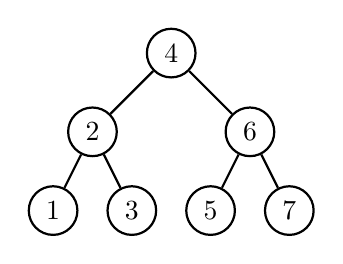
\begin{tikzpicture}[thick, 
	level 1/.style={sibling distance=2cm},
	level 2/.style={sibling distance=1cm},
	level 3/.style={sibling distance=0.5cm},
	level distance = 1cm
	]
\node [circle,draw] (n4){$4$}
  child {node [circle,draw] (n2) {$2$}
  	child {node [circle,draw] (n1) {$1$}}
  	child {node [circle,draw] (n3) {$3$}}
  }
  child {node [circle,draw] (n6) {$6$}
  	child {node [circle,draw] (n5) {$5$}}
  	child {node [circle,draw] (n7) {$7$}}
 };
%\tikzstyle{nodo}=[shape=circle,draw,thick,inner sep=0pt,minimum size=25pt,draw=black]
%\node [nodo] (n4) {$4$};
%\node [nodo] (n2) [below of=n4] {$2$};
%\node [nodo] (n6) [below of=n4] {$6$};
%\path (n4) edge [thick] (n2);
%\path (n4) edge [thick] (n6);
%\node [mode] (m1) [right of=t2] {{\large\bf R}};
%\path (m1) edge [thick] (t1);
%\node [task] (t5) [below of=t4] {{\large$t_5$}};
%\node [mode] (m3) [right of=t5] {{\large\bf RW}}
%edge [thick] (t5)
%edge [<-,thick] (m2);
\end{tikzpicture}
\caption{Exemplo de árvore de busca binária.}
\label{aula05:fig:arv}
\end{figure}

Os passos na operação de {\bf busca} para uma chave $x$ são:
\begin{enumerate}
\item Compare com a chave que está na raiz.
\item Se $x$ é menor, vá para a sub-árvore esquerda.
\item Se $x$ é maior, vá para a sub-árvore direita.
\item Repita o processo recursivamente, até que a chave procurada seja
encontrada ou um nó folha é atingido.
\end{enumerate}
O algoritmo de busca em árvore binária é ilustrado na figura~\ref{aula05:algo:arv:busca}.
\begin{figure}[!htb]
\centering
\begin{framed}
\begin{lstlisting}
Arv* ArvBusca( Arv* a, int chave ) {
	if( a == NULL )        return NULL;
	if( a.chave == chave)  return a;
	if( chave < a.chave )  return ArvBusca( a->esq, chave );
	else                   return ArvBusca( a->dir, chave );
	return NULL;
}
\end{lstlisting}
\end{framed}
\caption{Algoritmo de busca em árvore binária.}
\label{aula05:algo:arv:busca}
\end{figure}

O procedimento de {\bf inserção} é:
\begin{enumerate}
\item Executar o procedimento de busca da chave a ser inserida.
\item O ponto onde deveria estar a chave é o ponto de inserção.
\end{enumerate}

O procedimento de {\bf remoção} não é tão simples:
\begin{enumerate}
\item Executar o procedimento de busca da chave a ser removida.
\item Se o nó contém o registro a ser removido possui no máximo
um descendente, trocar o nó a ser removido pelo seu descendente.
\item Se possuir dois descendentes o registro a ser removido deve ser primeiro
substituído:
	\begin{itemize}
	\item pelo registro mais à direita na sub-árvore esquerda.
	\item ou pelo registro mais à esquerda na sub-árvore direita.
	\end{itemize}
\end{enumerate}

{\bf Análise} -- o número de comparações em uma busca com sucesso no melhor caso é 
$C(n)= 1$, pior caso $C(n) = n$ e caso médio $C(n) = \log  n$.
O pior caso ocorre quando as chaves são inseridas em ordem crescente ou decrescente.

%%%%%%%%%%%%%%%%%%%%%%%%%%%%%%%%%%%%%%%%%%%%%%%%%%%%%%%%%%%%%%%%%%%%%%%%%%%%%%%
\section{Propriedades em árvores}
%%%%%%%%%%%%%%%%%%%%%%%%%%%%%%%%%%%%%%%%%%%%%%%%%%%%%%%%%%%%%%%%%%%%%%%%%%%%%%%

%%%%%%%%%%%%%%%%%%%%%%%%%%%%%%%%%%%%%%%%%%%%%%%%%%%%%%%%%%%%%%%%%%%%%%%%%%%%%%%
\subsection{Percurso em árvores}

Há três tipos de percurso em árvores:
\begin{description}
\item[Pré-ordem -] o nó é visitado antes das sub-árvores descendentes. 
\item[Pós-ordem -] o nó é visitado depois das sub-árvores descendentes.
\item[Em-ordem -] em árvores binárias, o nó é visitado depois da sub-árvore
da esquerda e antes da sub-árvore da direita.
\end{description}

%%%%%%%%%%%%%%%%%%%%%%%%%%%%%%%%%%%%%%%%%%%%%%%%%%%%%%%%%%%%%%%%%%%%%%%%%%%%%%%
\subsection{Propriedades em árvores binárias}

Dada a notação:
\begin{itemize}
\item $n$ - número de nós.
\item $e$ - número de nós externos (folhas).
\item $i$ - número de nós internos (não folhas).
\item $h$ - altura.
\end{itemize}
Segue as seguintes propriedades sobre árvores binárias:
\begin{itemize}
\item $e = i + 1$.
\item $n = 2e - 1$.
\item $h \leq i$.
\item $h \leq (n-1)/2$.
\item $e \leq 2^h$.
\item $h \geq \log e$.
\item $ \geq \log (n+1) -1$.
\end{itemize}



%%%%%%%%%%%%%%%%%%%%%%%%%%%%%%%%%%%%%%%%%%%%%%%%%%%%%%%%%%%%%%%%%%%%%%%%%%%%%%%
\section{Árvores de busca balanceadas}
%%%%%%%%%%%%%%%%%%%%%%%%%%%%%%%%%%%%%%%%%%%%%%%%%%%%%%%%%%%%%%%%%%%%%%%%%%%%%%%

Uma limitação das árvores binárias de pesquisa é a ordem em que os elementos
são inseridos. Por exemplo, as ordens de inserção abaixo:
\begin{itemize}
\item ordem $1, 2, 3, 4, 5, 6, 7$ gera uma {\bf árvore degenerada} (todo nó
tem apenas um filho).
\item ordem $4, 6, 2, 5, 1, 7, 3$ gera uma árvore binária completa.
\end{itemize}
O que afeta diretamente o desempenho na busca de elementos.

Idealmente deseja-se que a árvore esteja {\bf completamente balanceada}.
A distância média para qualquer nó da árvore é mínima.
No entanto, manter uma árvore completamente balanceada tem alto custo.
Uma solução é procurar uma solução intermediária que possa manter a árvore
balanceada.

Uma {\bf árvore de busca balanceada} garante uma altura de $O(\log n)$
quando implementa um conjunto dinâmico de $n$ itens.
Alguns exemplos de árvores balanceadas são AVL, árvores 2-3, árvores 2-3-4,
B-trees e árvore rubro-negra.

%%%%%%%%%%%%%%%%%%%%%%%%%%%%%%%%%%%%%%%%%%%%%%%%%%%%%%%%%%%%%%%%%%%%%%%%%%%%%%%
\subsection{Árvore AVL}

Uma árvore binária é denominada {\bf AVL} (dos seus criados Georgy
Adelson-Velsky e Landis) se para todos os nós, {\bf as alturas de suas duas
sub-árvores diferem no máximo em uma unidade}, sendo assim balanceada.
Operações de consulta, inserção e remoção de nós tem custo $O(\log n)$.

O {\bf fator de balanceamento} (FB) de um nó é a diferença entre
a altura da sub-árvore da esquerda e a altura da sub-árvore da direita.
Se não existir uma sub-árvore, a altura é zero.
Os resultados de um FB são:
\begin{itemize}
\item $> 0$ - sub-árvore da direita é menor.
\item $< 0$ - sub-árvore da esquerda é menor.
\item $= 0$ - sub-árvores tem a mesma altura.
\end{itemize}
Os valores válidos de FB são $-1$ (sub-árvore da esquerda é menor), $0$, $1$
(sub-árvore da direita é menor).

\subsubsection{Inserção}

O nó é inserido como em uma árvore binária comum.
Se a inserção não degenerar a árvore, o processo termina.
Caso contrário, é necessário:
\begin{enumerate}
\item encontrar o nó cujo FB esteja fora do intervalo (pivô).
\item realizar uma rotação na árvore a partir do nó ``pivô''
(rotação simples ou rotação dupla).
\end{enumerate}
Apenas uma rotação (simples ou dupla) é necessária.
Após essa rotação, a árvore já estará balanceada.
Há quatro possibilidades de rotão:
\begin{itemize}
\item 2 casos externos (direita e esquerda) com rotação simples.
\item 2 casos internos (direta e esquerda) com rotação dupla.
\end{itemize}

\subsubsection{Rotação}

Suponha que $\alpha$ seja um pivô, nos casos externos, uma rotação simples é necessária 
caso a inserção ocorra na \textbf{sub-árvore à esquerda do filho à esquerda de} $\alpha$
ou na \textbf{sub-árvore à direita do filho à direita de} $\alpha$.
A figura~\ref{aula05:avl:rot:simples1} demonstra dois exemplos de rotação
simples a direta.
%
\begin{figure}[!htb]
\centering
  \begin{minipage}{0.2\textwidth}
	\centering
	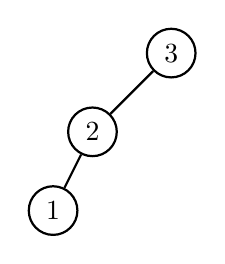
\begin{tikzpicture}[thick, 
		level 1/.style={sibling distance=2cm},
		level 2/.style={sibling distance=1cm},
		level 3/.style={sibling distance=1cm},
		level distance = 1cm
		]
	\node [circle,draw] (n3) {3}
	  child {
		node [circle,draw] (n2) {2}
			child { node [circle,draw] (n1) {1} }
			child[missing] {}
	  }
	  child[missing] {};
	\end{tikzpicture}
  \end{minipage}
%
  \begin{minipage}{0.2\textwidth}
	\centering
	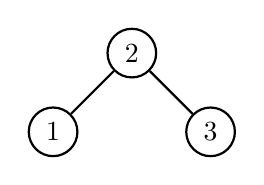
\begin{tikzpicture}[thick, 
		level 1/.style={sibling distance=2cm},
		level 2/.style={sibling distance=1cm},
		level 3/.style={sibling distance=1cm},
		level distance = 1cm
		]
	\node [circle,draw] (n2) {2}
		child { node [circle,draw] (n1) {1} }
		child { node [circle,draw] (n3) {3} };
	\end{tikzpicture}
  \end{minipage}
  %
  \vline
  %
  \begin{minipage}{0.25\textwidth}
	\centering
	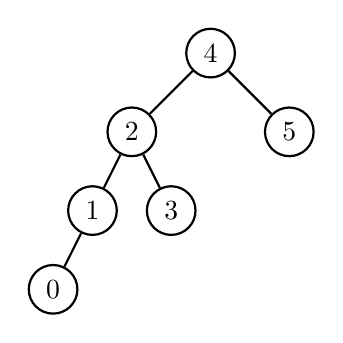
\begin{tikzpicture}[thick,
		level 1/.style={sibling distance=2cm},
		level 2/.style={sibling distance=1cm},
		level 3/.style={sibling distance=1cm},
		level distance = 1cm ]
	\node [circle,draw] (n4) {4}
	  child {
		node [circle,draw] (n2) {2}
		child {
			node [circle,draw] (n1) {1}
			child { node[circle,draw] (n0) {0} }
			child[missing] {}
		}
		child { node[circle,draw] (n3) {3} }
	  }
	  child { node [circle,draw] (n5) {5} };
	\end{tikzpicture}
  \end{minipage}
%
  \begin{minipage}{0.2\textwidth}
	\centering
	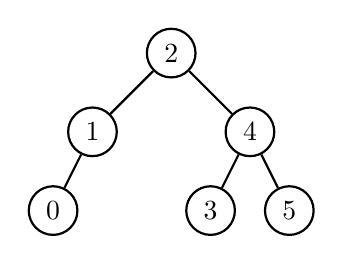
\begin{tikzpicture}[thick,
		level 1/.style={sibling distance=2cm},
		level 2/.style={sibling distance=1cm},
		level 3/.style={sibling distance=1cm},
		level distance = 1cm ]
	\node [circle,draw] (n2) {2}
	  child {
		node [circle,draw] (n1) {1}
		child { node [circle,draw] (n0) {0} }
		child[missing] {}
	  }
	 child {
		 node[circle,draw] (n4) {4}
		child { node [circle,draw] (n3) {3} }
		child { node [circle,draw] (n5) {5} }
	 };
	\end{tikzpicture}
  \end{minipage}
\caption{Dois exemplos de AVL com rotação simples para a direita.}
\label{aula05:avl:rot:simples1}
\end{figure}

Nos casos internos, suponha que o pivô seja $\alpha$, 
uma rotação dupla é necessária caso a inserção ocorra 
na {\bf sub-árvore à esquerda do filho à direita de} $\alpha$ ou
na {\bf sub-árvore à direita do filho à esquerda de} $\alpha$.
Uma rotação dupla equivale a duas rotações simples em sequência.
A figura~\ref{aula05:avl:rot:dupla1} demonstra um exemplo de rotação
dupla a direta.
%
\begin{figure}[!htb]
\centering
  \begin{minipage}{0.3\textwidth}
	\centering
	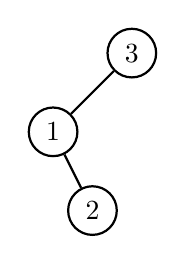
\begin{tikzpicture}[thick, 
		level 1/.style={sibling distance=2cm},
		level 2/.style={sibling distance=1cm},
		level 3/.style={sibling distance=1cm},
		level distance = 1cm
		]
	\node [circle,draw] (n3) {3}
	  child {
		node [circle,draw] (n1) {1}
			child[missing] {}
			child { node [circle,draw] (n2) {2} }
	  }
	  child[missing] {};
	\end{tikzpicture}
  \end{minipage}
%
  \vline
%
  \begin{minipage}{0.3\textwidth}
	\centering
	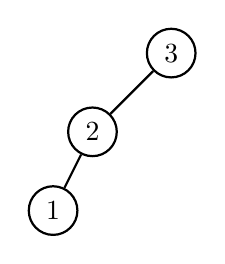
\begin{tikzpicture}[thick, 
		level 1/.style={sibling distance=2cm},
		level 2/.style={sibling distance=1cm},
		level 3/.style={sibling distance=1cm},
		level distance = 1cm
		]
	\node [circle,draw] (n3) {3}
	  child {
		node [circle,draw] (n2) {2}
			child { node [circle,draw] (n1) {1} }
			child[missing] {}
	  }
	  child[missing] {};
	\end{tikzpicture}
  \end{minipage}
%
  \vline
%
  \begin{minipage}{0.3\textwidth}
	\centering
	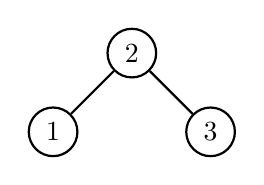
\begin{tikzpicture}[thick, 
		level 1/.style={sibling distance=2cm},
		level 2/.style={sibling distance=1cm},
		level 3/.style={sibling distance=1cm},
		level distance = 1cm
		]
	\node [circle,draw] (n2) {2}
		child { node [circle,draw] (n1) {1} }
		child { node [circle,draw] (n3) {3} };
	\end{tikzpicture}
  \end{minipage}
\caption{Exemplo de AVL com rotação dupla.}
\label{aula05:avl:rot:dupla1}
\end{figure}

\subsubsection{Remoção}

A remoção em AVL é similar a inserções, mas mais complexas.
Incialmente, usa-se a estratégia de remoção das árvores não balanceadas.
Porém, pode gerar desequilíbrio e exigir balanceamento.
Rotações simples e duplas são necessárias durante esse balanceamento.

Após o balanceamento, pode haver desequilíbrio em níveis superiores.
Assim, deve-ser analisar também esses níveis superiores.
A figura~\ref{aula05:avl:rm:ex1} demonstra um exemplo de remoção
com rotação simples a esquerda.
%
\begin{figure}[!htb]
\centering
  \begin{minipage}{0.3\textwidth}
	\centering
	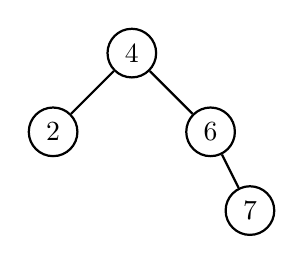
\begin{tikzpicture}[thick, 
		level 1/.style={sibling distance=2cm},
		level 2/.style={sibling distance=1cm},
		level 3/.style={sibling distance=1cm},
		level distance = 1cm
		]
	\node [circle,draw] (n4) {4}
	  child { node [circle,draw] (n2) {2} }
	  child {
		node [circle,draw] (n6) {6}
			child[missing] {}
			child { node [circle,draw] (n7) {7} }
	  };
	\end{tikzpicture}
  \end{minipage}
%
  \vline
%
  \begin{minipage}{0.3\textwidth}
	\centering
	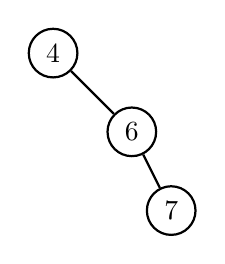
\begin{tikzpicture}[thick, 
		level 1/.style={sibling distance=2cm},
		level 2/.style={sibling distance=1cm},
		level 3/.style={sibling distance=1cm},
		level distance = 1cm
		]
	\node [circle,draw] (n4) {4}
	  child[missing] {}
	  child {
		node [circle,draw] (n6) {6}
			child[missing] {}
			child { node [circle,draw] (n7) {7} }
	  };
	\end{tikzpicture}
  \end{minipage}
%
  \vline
%
  \begin{minipage}{0.3\textwidth}
	\centering
	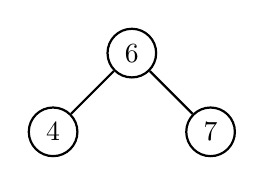
\begin{tikzpicture}[thick, 
		level 1/.style={sibling distance=2cm},
		level 2/.style={sibling distance=1cm},
		level 3/.style={sibling distance=1cm},
		level distance = 1cm
		]
	\node [circle,draw] (n6) {6}
		child { node [circle,draw] (n4) {4} }
		child { node [circle,draw] (n7) {7} };
	\end{tikzpicture}
  \end{minipage}
\caption{Exemplo de remoção em AVL (nó 2) com rotação simples a esquerda.}
\label{aula05:avl:rm:ex1}
\end{figure}

\subsubsection{Análise}

Entre as possíveis operações temos:
\begin{itemize}
\item {\bf rotação} única custo $O(1)$ pois é constante.
\item {\bf busca}  é $O(\log n)$ pois a altura de árvore é $O(\log n)$
e não necessita balanceamento.
\item {\bf inserção} é $O(\log n)$ com o custo da busca incial de $O(\log n)$
e mais balanceamento para manter FP tem custo $O(\log n)$.
\item {\bf remoção} é $O(\log n)$ com a busca inicial de $O(\log n)$ mais
balanceamento para manter FP tem custo $O(\log n)$.
\end{itemize}

%%%%%%%%%%%%%%%%%%%%%%%%%%%%%%%%%%%%%%%%%%%%%%%%%%%%%%%%%%%%%%%%%%%%%%%%%%%%%%%
\subsection{Árvore rubro-negra}

\todo[inline]{Prox. aula.}

%%%%%%%%%%%%%%%%%%%%%%%%%%%%%%%%%%%%%%%%%%%%%%%%%%%%%%%%%%%%%%%%%%%%%%%%%%%%%%%
\subsection{Árvore SBB}

\todo[inline]{Prox. aula.}

%%%%%%%%%%%%%%%%%%%%%%%%%%%%%%%%%%%%%%%%%%%%%%%%%%%%%%%%%%%%%%%%%%%%%%%%%%%%%%%
\section{Tabelas \textsc{Hash}}
%%%%%%%%%%%%%%%%%%%%%%%%%%%%%%%%%%%%%%%%%%%%%%%%%%%%%%%%%%%%%%%%%%%%%%%%%%%%%%%

\todo[inline]{Prox. aula.}

%%%%%%%%%%%%%%%%%%%%%%%%%%%%%%%%%%%%%%%%%%%%%%%%%%%%%%%%%%%%%%%%%%%%%%%%%%%%%%%
\section{Exercícios}
%%%%%%%%%%%%%%%%%%%%%%%%%%%%%%%%%%%%%%%%%%%%%%%%%%%%%%%%%%%%%%%%%%%%%%%%%%%%%%%

\begin{enumerate}
\item Descreva os passos da busca binária e os custos para o melhor caso, caso médio
e pior caso.

\item Escreva o algoritmo para imprimir o \textsc{menor} elemento de uma árvore de busca binária.
\item Escreva o algoritmo para imprimir o \textsc{maior} elemento de uma árvore de busca binária.
\end{enumerate}
